% This file was created by matlab2tikz.
%
%The latest updates can be retrieved from
%  http://www.mathworks.com/matlabcentral/fileexchange/22022-matlab2tikz-matlab2tikz
%where you can also make suggestions and rate matlab2tikz.
%
\documentclass[tikz]{standalone}
\usepackage[T1]{fontenc}
\usepackage[utf8]{inputenc}
\usepackage{pgfplots}
\usepackage{grffile}
\pgfplotsset{compat=newest}
\usetikzlibrary{plotmarks}
\usepgfplotslibrary{patchplots}
\usepackage{amsmath}
\usetikzlibrary{decorations.markings}
\usetikzlibrary{decorations, decorations.text,backgrounds}
\usetikzlibrary{spy}
\usetikzlibrary{shapes.misc}
\usetikzlibrary{external}
\usetikzlibrary{backgrounds}

\tikzset{cross/.style={cross out, draw=black, minimum size=2*(#1-\pgflinewidth), inner sep=0pt, outer sep=0pt},cross/.default={1pt}}

\begin{document}

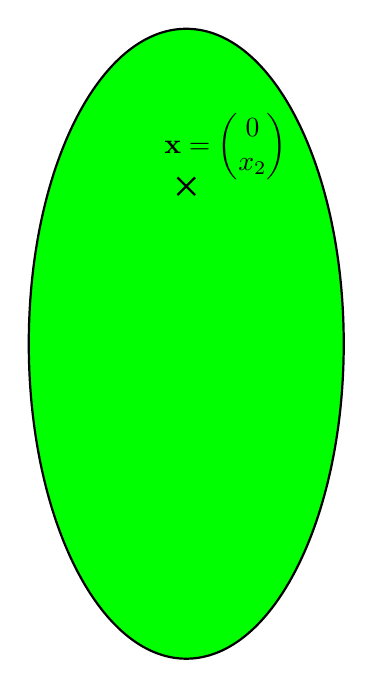
\begin{tikzpicture}
	\draw[white](0,-2) -- (1.5,-2);
	\draw[thick,fill=green] (0,0) circle [x radius=2, y radius = 4];
	\draw[thick] (0,2) node[cross=4pt] {};
	\draw(0.5,2.5) node {$\mathbf{x} =\begin{pmatrix}0\\ x_2\end{pmatrix}$};
\end{tikzpicture}
\end{document}